\section{Elliptic Curves}\label{Chapter: Elliptic Curves}

As discussed in the introduction, the aim of the thesis is to give a formal overview of the proof of one of the most celebrated problems(now a Theorem) in Mathematics, Fermat's last theorem, due to Prof. Dr. Andrew Wiles in 1995. Elliptic curves have been one of the central and key objects in the proof of  Fermat's last theorem. Sir Andrew Wiles proved in his paper that all semistable elliptic curves over the set of rational numbers $\Q$ are modular. Fermat’s Last theorem follows as a corollary by virtue of previous work by Frey, Serre and Ribet. Thus it is important that we begin by introducing the building blocks and the objects of the proof and study certain aspects revolving around them which are important to completely understand the proof. 

We will closely follow the book \cite{diamond2005first} and Lecture notes from Marc Masdeu, \cite{Masdeu2015ModularForms} , \cite{bostonFermat}, \cite{silv}.  We will sometimes closely follow proofs from either of these sources for the sake of completeness. At times the ideas of the proofs are not original, neither I want to claim so, although, at some places,  I have expanded on my own giving more details.  

We will start with defining double coset operators, a notion that lies as a key concept in the background of theory. 
At times, the ideas are inevitably not original but closely followed.


\subsection{Weierstrass Equations}
 The Weierstrass equation is a fundamental equation in the theory of elliptic curves. It provides a standard form for elliptic curves over a field (often over the complex numbers, but also over other fields like the reals or rationals).
\begin{definition}
 The general Weierstrass equation over a field $k$ is given by:

\[ y^2 + a_1xy + a_3y = x^3 + a_2x^2 + a_4x + a_6 \] where, \( a_1, a_2, a_3, a_4, \) and \( a_6 \) are coefficients lying in the given field $k$.
\end{definition}

\begin{remark}
The equation defines a cubic curve in the projective plane.
\end{remark}
\begin{definition}[Elliptic Curves]
An elliptic curve $(E, O)$ over a field $k$ is a smooth, projective curve $E$ of genus 1 along with a specified point $O$ known as the base point, all defined over $k$. \\
\end{definition}
 
 \begin{remark}
   $O$ is usually understood as the base point, and thus we will denote an elliptic curve defined over a field $k$ by $E$  instead of $(E, O)$. Furthermore, the non-singularity or smoothness just means that the curve has no cusps or self-intersections.
 \end{remark} 

 The following proposition gives the exact connection between Weierstrass equations and elliptic curves. 
 
\begin{proposition}\label{1.1.5}
    Let $E$ be an elliptic curve. Then there exist coordinate functions $x, y \in k(E)$ and constants $a_{1}, a_{2}, a_{3}, a_{4}, a_{6} \in k$ such that the following condition holds: \\
    If $f: E \rightarrow \mathbb{P}^{2}_k$ is the map given by $P \mapsto[x(P): y(P): 1]$, then $f$ gives an isomorphism of elliptic curves(understanding where the base point is mapped to) between $E$ and the curve $Y^{2}+a_{1} X Y+a_{3} Y=X^{3}+a_{2} X^{2}+a_{4} X+a_{6}$. Conversely, every such equation gives an elliptic curve with base point $O=[0:1:0]$ whenever it is smooth.
\end{proposition}
\begin{proof}
    See, in section 4.2 in this thesis.
\end{proof}

First, let us restrict to the affine case and consider a Weierstrass equation, 

\begin{equation}
    y^2 + a_1xy + a_3y = x^3 + a_2x^2 + a_4x + a_6.
\end{equation}


\subsection{Simplified Weierstrass equation, Examples}

In this section, we'll focus on the affine case, using the non-homogeneous coordinates \( x \) and \( y \). It's important to remember that in this setting, there's always a point at infinity, denoted as \( O=[0:1:0] \).

Let's take a closer look at a Weierstrass equation, which we'll call \( E \). If the characteristic of the field \( k \) is not 2, we can simplify the equation by completing the square. This is done by introducing a new variable, \( \eta \), defined as:

\[
\eta = y + \frac{a_1 x + a_3}{2}.
\]

Using this transformation, \( E \) can be rewritten as:

\[
\eta^2 = x^3 + \frac{b_2}{4}x^2 + \frac{b_4}{2}x + \frac{b_6}{4},
\]

where the coefficients \( b_2 \), \( b_4 \), and \( b_6 \) are defined as \( b_2 = a_1^2 + 4a_2 \), \( b_4 = a_1a_3 + 2a_4 \), and \( b_6 = a_3^2 + 4a_6 \), respectively.

Similarly, if the characteristic of \( k \) is not 3, we can complete the cube by introducing another variable, \( \xi \), defined as \( \xi = x + \frac{b_2}{12} \). This transforms the equation into:

\[
\eta^2 = \xi^3 - \frac{c_4}{48}\xi - \frac{c_6}{864},
\]

where \( c_4 = b_2^2 - 24b_4 \) and \( c_6 = -b_2^3 + 36b_2b_4 - 216b_6 \).

Additionally, we define two more quantities:

\[
b_8 = a_1^2a_6 - a_1a_3a_4 + 4a_2a_6 + a_2a_3^2 - a_4^2
\]
and
\[
\Delta = -b_2^2b_8 - 8b_4^3 - 27b_6^2 + 9b_2b_4b_6.
\]
\begin{definition}
The quantity  \( \Delta \) is called the discriminant of a Weierstrass equation. \\
The \( j \)-invariant of the elliptic curve \( E \) is defined as:

\[
j = \frac{c_4^3}{\Delta}.
\]    
\end{definition}


The discriminant \( \Delta \) is a crucial parameter in understanding the nature of the elliptic curve \( E \), and the \( j \)-invariant is a key characteristic that helps classify the curve.

Furthermore, when the characteristic of \( k\) is neither 2 nor 3, using suitable transformations, any Weierstrass equation in the form of \( \eta^2 = x^3 + \ldots \) can be simplified to a more manageable form:

\[
y^2 = x^3 - 27c_4x - 54c_6.
\]

This leads us to what is known as the simplified Weierstrass form:

\[
y^2 = x^3 + ax + b.
\]

This simplified form is easier to work with and forms the basis for many further investigations in the study of elliptic curves.\\

Next, we give a proposition that characterises the discriminant of a Weierstrass equation and provides a lovely connection between j-invariants and elliptic curves.

\begin{proposition}
Let $E$ be a curve given by a Weierstrass equation. Then, \newline
$E$ is non-singular if and only if \textbf{$\Delta \neq 0$}.

\newline
\begin{proof} 

Consider an elliptic curve \( E \) defined by the Weierstrass equation:

\[
E: y^2 + a_1xy + a_3y = x^3 + a_2x^2 + a_4x + a_6.
\]

Our first goal is to demonstrate that the point at infinity is not a singular point on this curve. To do this, we extend the equation into the projective plane \( \mathbb{P}^2 \) by introducing a homogenized form of the equation:

\[
F(X, Y, Z) = Y^2Z + a_1XYZ + a_3YZ^2 - X^3 - a_2X^2Z - a_4XZ^2 - a_6Z^3 = 0.
\]

We focus on the point at infinity, \( O = [0:1:0] \). Calculating the partial derivative of \( F \) with respect to \( Z \) at \( O \) gives us:

\[
\frac{\partial F}{\partial Z}(O) = 1 \neq 0.
\]

This result, according to the Projective Jacobi criterion, confirms that \( O \) is indeed a non-singular point on \( E \).

Now, let's suppose that \( E \) has a singular point, denoted as \( P_0 = (x_0, y_0) \). By shifting coordinates:

\[
x = x' + x_0, \quad y = y' + y_0,
\]

we note that after doing tedious and straight forward computations the discriminant \( \Delta \) and \( c_4 \) remain unchanged. Therefore, we can assume, without loss of generality, that \( E \) is singular at the origin \( (0,0) \). This leads us to deduce that:

\[
a_6 = f(0,0) = 0, \quad a_4 = \frac{\partial f}{\partial x}(0,0) = 0, \quad a_3 = \frac{\partial f}{\partial y}(0,0) = 0.
\]

Consequently, the equation for \( E \) simplifies to:

\[
E: y^2 + a_1xy - a_2x^2 - x^3 = 0,
\]

from which it follows that \( \Delta = 0 \).

Conversely, assuming that the characteristic of the field \( k \) is not 2, let's consider a Weierstrass equation in the form:

\[
y^2 = 4x^3 + b_2x^2 + 2b_4x + b_0.
\]

It can be shown that the curve associated with this equation is singular if and only if it has a double point of the form \( (x_0, 0) \). This condition is equivalent to the vanishing of the discriminant, which is \( 16\Delta \) in this case.
\\
A similar approach can be employed for charachteristic 2 and 3. For more details see, \cite{silv}
\end{proof}
\end{proposition} 
 
 \begin{proposition}
     Two elliptic curves $E, E'$ are isomorphic (over $\bar{k}$ ) if and only if they have the same $\bm{j}$\textbf{-invariant}.
\begin{proof}
 It is clear that if $E$ \text{and} $E'$ are isomorphic over $\overline{k}$, we get that their \textit{j-invariants} are equal. This is due to the fact that, we can get weierstrass equations assosciated with them and establish a transformation, which maps one equation to the other. It can be noted that, since the quantities $c_4, \Delta$ remain invariant under such transformations and so do their j-invariants. \\
 
 Conversely, again for simplicity, assume $char(k)\neq 2,3$, and thus as per the discussion above, we get a simplified Weierstrass equation of the form $y^2=x^3+ax+b$. \newline
 In this case, we get that $\Delta=-16(4a^3+27b^2)$ and $j=-1728 \frac{64a^3}{\Delta}$. \\
 Let $E: y^2=x^3+ax+b \newline E': y^2=x^3+Ax+B$.
 Assume that their j-invariants are equal, but then by the above definitions, we get that $a^3B^2=A^3b^2$. 
 Now, we make a case distinction: \\
case 1) If $a=0$, it is clear that since an Elliptic curve is non-singular and by part (a) $\Delta \neq 0 $ forces that $A=0$ and thus we get that $(x,y)  \mapsto (c^2x,c^3y)$ where $c=(\frac{b}{B})^\frac{1}{6}$ gives an isomorphism between $E$ and $E'$ (over $\overline{k}$). Note here we use that the isomorphism is over $\overline{k}$ to get such a $c$. \\
Case 2) By symmetry, the case $b=0$ can be handled analogously. \\
Case 3) When $ab \neq 0$, then, it is clear that $AB \neq 0$, thus we have that $(\frac{a}{A})^\frac{1}{4}=(\frac{b}{B})^\frac{1}{6}$, thus chose $c=(\frac{a}{A})^\frac{1}{4}$ as in case 1), we get an isomorphism between $E$ and $E'$ (over $\overline{k}$) \newline
For more details and for proof in $char(k)=2$, see \cite{silv}   
\end{proof}
 \end{proposition}\newline

Now that we have seen important quantities associated with the Weierstrass equation and elliptic curves we give some examples.\\
Note that for plotting curves, I used \href{https://www.desmos.com/}{DESMOS}
\begin{example}
  1)  Consider the Weierstrass equation $y^2=x^3-4x+2$, with the real plot below,
  \begin{center}
      \includegraphics[width=0.47\textwidth]{desmos-graph (6).png}
  \end{center}
    
Let us calculate some of the quantities mentioned above:
$\Delta=-16(4a^3+27b^2)$ and thus, substituting values of $a,b$ we get that, \\ 
$\Delta=-16(4(-4)^3+27(2)^2)$ , i.e, \\
$\Delta=2368$.\\Similarly, we know that 
$j=-1728 \frac{64a^3}{\Delta}$,\\
thus again substituting values of $a,b, \Delta$ we get that,\\
$j=-1728 \frac{64(-4)^3}{2368}$.




2)  Consider the Weierstrass equation $y^2=x^3-2x+2$, with the real plot below:
\begin{center}
     \includegraphics[width=0.47\textwidth]{desmos-graph (5).png}
\end{center}
 \end{example}  
\\
\subsection{Complex Tori and Elliptic curves}

This section defines basic terminologies like Lattices, Complex tori, etc, and states and proves some results related to them. Furthermore, the main aim of this section is to state the correspondence between Complex Tori and Elliptic curves. 
\begin{definition}[Complex lattice]
    A \textit{complex lattice} $\Lambda$ is a set of the form $\mathbb{Z}\Lambda_1 \oplus \mathbb{Z}\Lambda_2$ such that \\
    I) $\Lambda_1, \Lambda_2 \in \mathbb{C}$, \\
    II) The set $\{\Lambda_1, \Lambda_2\}$ forms a $\mathbb{R}$- basis of $\mathbb{C}$. 
\end{definition}
For example, the set of Gaussian integers $\mathbb{Z}[i]= \{a+bi : a, b \in \mathbb{Z} \}$ is a complex lattice. \\

Let $\mathcal{H}= \{ z \in \mathbb{C} : Im(z) > 0 \}$ denote the complex upper half plane. We begin with a small lemma.
\begin{lemma}
Consider two lattices $\Lambda=\Lambda_{1} \mathbb{Z} \oplus \Lambda_{2} \mathbb{Z}$ and $\Lambda^{\prime}=\Lambda_{1}^{\prime} \mathbb{Z} \oplus \Lambda_{2}^{\prime} \mathbb{Z}$ with $\Lambda_{1} / \Lambda_{2} \in \mathcal{H}$ and $\Lambda_{1}^{\prime} / \Lambda_{2}^{\prime} \in \mathcal{H}$. Then $\Lambda^{\prime}=\Lambda$ if and only if

$$
\left[\begin{array}{l}
\Lambda_{1}^{\prime} \\
\Lambda_{2}^{\prime}
\end{array}\right]=\left[\begin{array}{ll}
a & b \\
c & d
\end{array}\right]\left[\begin{array}{l}
\Lambda_{1} \\
\Lambda_{2}
\end{array}\right] \quad \text { for some }\left[\begin{array}{ll}
a & b \\
c & d
\end{array}\right] \in \mathrm{SL}_{2}(\mathbb{Z}) .
$$
\begin{proof}

Suppose there exists a matrix \( \left[\begin{array}{cc} a & b \\ c & d \end{array}\right] \) in \(\mathrm{SL}_2(\mathbb{Z})\) such that,

\[ \left[\begin{array}{c} \Lambda_1' \\ \Lambda_2' \end{array}\right] = \left[\begin{array}{cc} a & b \\ c & d \end{array}\right] \left[\begin{array}{c} \Lambda_1 \\ \Lambda_2 \end{array}\right]. \]

This just implies that each basis vector of \(\Lambda'\) can be expressed as an integer linear combination of the basis vectors of \(\Lambda\). Since the matrix is in \(\mathrm{SL}_2(\mathbb{Z})\), its determinant is 1, and it is invertible with its inverse also having integer entries. This means that there exists a matrix $A^{-1}=$\( \left[\begin{array}{cc} a' & b' \\ c' & d' \end{array}\right] \) in \(\mathrm{SL}_2(\mathbb{Z})\) such that,

\[ \left[\begin{array}{c} \Lambda_1 \\ \Lambda_2 \end{array}\right] = \left[\begin{array}{cc} a' & b' \\ c' & d' \end{array}\right] \left[\begin{array}{c} \Lambda_1' \\ \Lambda_2' \end{array}\right]. \]

Similarly, as above this just means that each basis vector of \(\Lambda\) can be expressed as an integer linear combination of the basis vectors of \(\Lambda'\). \\
Thus, we get both the containments, $\Lambda \subset \Lambda'$ and $\Lambda' \subset \Lambda$, proving that, \(\Lambda' = \Lambda\).\\

Now, assume \(\Lambda' = \Lambda\). This means every vector in \(\Lambda'\) can be expressed as a linear combination of the basis vectors of \(\Lambda\), and vice versa. In terms of matrices, this means that there exist matrices $A,B$ with entries in the ring of integers $\Z$, such that \[ \left[\begin{array}{c} \Lambda_1 \\ \Lambda_2 \end{array}\right] = A \left[\begin{array}{c} \Lambda_1' \\ \Lambda_2' \end{array}\right], \]

\[ \left[\begin{array}{c} \Lambda_1' \\ \Lambda_2' \end{array}\right] = B\left[\begin{array}{c} \Lambda_1 \\ \Lambda_2 \end{array}\right]. \]

From, this we get that, 

\[ \left[\begin{array}{c} \Lambda_1 \\ \Lambda_2 \end{array}\right] = AB \left[\begin{array}{c} \Lambda_1\\ \Lambda_2 \end{array}\right]. \]

We claim that $AB=I$, where $I$ denote the $2X2$ identity matrix. 

Since $A,B$ are matrices with entries from $\Z$, it is clear that $AB$ has integer entries. Let $$A´B=\left[\begin{array}{cc} a & b \\ c & d \end{array}\right].$$
Then, from above, we have,

$(a-1)\Lambda_1+b\Lambda_2=0$ and similarly, $c\Lambda_1+(d-1)\Lambda_2=0$. 

Recall that $\Lambda_1, \Lambda_2$ generate a lattice and thus they are linearly independent over the real numbers. This implies that, $a-1=b=c=d-1=0$. Thus $AB=I$. 

This gives that det($A$)=det($B$)=$\pm.1$\\

But, it can be shown that $$\operatorname{Im}(\frac{\Lambda_1'}{\Lambda_2'})=k.\operatorname{det}(A)\operatorname{Im}.(\frac{\Lambda_1}{\Lambda_2}),$$ for some positive constant $k$. \\
Due to our assumption that $\Lambda_{1} / \Lambda_{2} \in \mathcal{H}$ and $\Lambda_{1}^{\prime} / \Lambda_{2}^{\prime} \in \mathcal{H}$, we have that $\operatorname{det}(A)=1$, giving us the desired matrix in $\mathrm{SL}_{2}(\mathbb{Z})$ .


\end{proof}
\end{lemma}

\begin{remark}
Note that, the assumption that $\Lambda_{1} / \Lambda_{2} \in \mathcal{H}$ and $\Lambda_{1}^{\prime} / \Lambda_{2}^{\prime} \in \mathcal{H}$, used above in the proof is really necessary for the statement above. For example, consider, the lattices spanned by \(1, i\) and \(1, -i\). They are equal, but the only matrix with integer entries \(A\) satisfying the above condition is \(A = \begin{pmatrix} 1 & 0 \\ 0 & -1 \end{pmatrix}\), which has determinant \(-1\). Note this happened since, $-i$ does not lie in the upper half plane as that $i$. 
\end{remark}

\begin{definition}[Complex Torus]    
A complex torus is a quotient of the complex plane by a lattice,
$$
\mathbb{C} / \Lambda=\{z+\Lambda: z \in \mathbb{C}\} .
$$
\end{definition}

\begin{remark}
 A complex torus algebraically is an Abelian group under the addition it inherits from $\mathbb{C}$ as its quotient. Let us try to visualise a complex torus geometrically. 
 Consider the lattice $\Lambda=\Lambda_{1} \mathbb{Z} \oplus \Lambda_{2} \mathbb{Z}$ and the assosciated torus $
\mathbb{C} / \Lambda$. It is a parallelogram spanned by $\left\{\Lambda_{1}, \Lambda_{2}\right\}$ with its sides identified in opposing pairs. Identifying one pair of sides rolls the parallelogram into a tube, and then identifying the other pair bends the tube into a torus. The following diagram explains this visually.
\begin{center}
    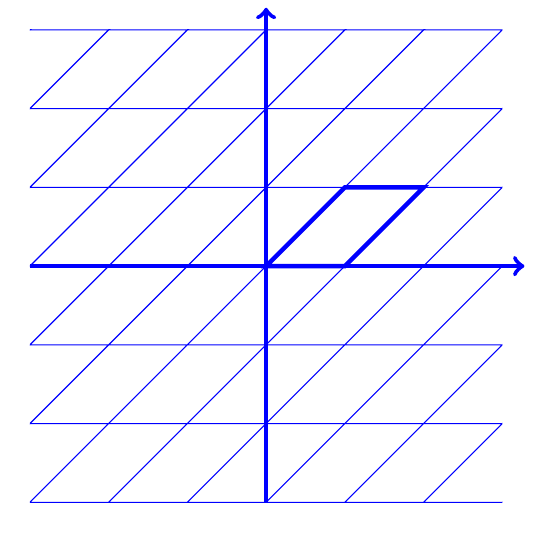
\begin{tikzpicture}[remember picture, blue]
\draw[->,ultra thick,shorten >=-8pt] (-3,0) -- (3,0);
\draw[->,ultra thick,shorten >=-8pt] (0,-3) -- (0,3);
\begin{scope}
\clip (-3,-3) rectangle (3,3);
\begin{scope}[xslant=1]
\draw (-6,-6) grid (6,6);
\draw[ultra thick] (0,0) rectangle (1,1);
\end{scope}
\end{scope}
\end{tikzpicture}
\begin{tikzpicture}[remember picture, blue]
\begin{scope}[xshift=1cm]
\draw[postaction={decorate},decoration={
    markings,
    mark=at position .145 with {\arrow{latex}},
    mark=at position .375 with {\arrow{latex}},
    mark=at position .395 with {\arrow{latex}},
    mark=at position .635 with {\arrowreversed{latex}},
    mark=at position .875 with {\arrowreversed{latex}},
    mark=at position .895 with {\arrowreversed{latex}}
    }
  ]
    (0,-1) -- +(2,0) -- +(2,2) -- +(0,2) -- cycle;
\end{scope}
\begin{scope}[xshift=4.5cm]
\draw[postaction={decorate},decoration={
    markings,
    mark=at position .5 with {\arrow{latex}}
    }
  ]
    (0,.25) -- ++(2,0);
\draw[postaction={decorate},decoration={
    markings,
    mark=at position .5 with {\arrow{latex}}
    }
  ]
    (0,-.25) -- ++(2,0);
\draw[postaction={decorate},decoration={
    markings,
    mark=at position .5 with {\arrow{latex}},
    mark=at position .55 with {\arrow{latex}}
    }
  ] (0,-.25) to[out=-120,in=0] (-.35,-.75) to[out=180,in=180] (-.35,.75) to[out=0,in=120] (0,.25);
\draw (2,.25) to[out=120,in=0] (1.65,.75) -- (-.35,.75) (-.35,-.75) --  (1.65,-.75) to[out=0,in=-120] (2,-.25);
\begin{scope}
\clip (0,.25) rectangle (2,-.25);
\draw[postaction={decorate},decoration={
    markings,
    mark=at position .5 with {\arrow{latex}},
    mark=at position .58 with {\arrow{latex}}
    }
  ]  (1.65,.75) to[out=180,in=180] (1.65,-.75);
\end{scope}
\begin{scope}[xshift=3cm]
\draw[postaction={decorate},decoration={
    markings,
    mark=at position .5 with {\arrow{latex}},
    }
  ]  (0,0) -- (2,0);
\draw[postaction={decorate},decoration={
    markings,
    mark=at position .5 with {\arrow{latex}},
    mark=at position .55 with {\arrow{latex}},
    }
  ] (0,0) arc[start angle=0,delta angle=-360,x radius=.35,y radius=.75];
\draw (2,0) arc[start angle=0,delta angle=-90,x radius=.35,y radius=.75] -- ++(-2,0);
\draw (2,0) arc[start angle=0,delta angle=90,x radius=.35,y radius=.75] -- ++(-2,0);
\end{scope}
\end{scope}
\begin{scope}[yshift=-3cm]
\draw[postaction={decorate},decoration={
    markings,
    mark=at position .5 with {\arrow{latex}},
    }
  ]  (0,0) -- (3,0);
\draw[postaction={decorate},decoration={
    markings,
    mark=at position .5 with {\arrow{latex}},
    mark=at position .6 with {\arrow{latex}},
    }
  ] (0,0) arc[start angle=0,delta angle=-360,x radius=.15,y radius=.35];
\draw (3,0) arc[start angle=0,delta angle=-90,x radius=.15,y radius=.35] -- ++(-3,0);
\draw (3,0) arc[start angle=0,delta angle=90,x radius=.15,y radius=.35] -- ++(-3,0);
\begin{scope}[xshift=4cm]
\draw[postaction={decorate},decoration={
    markings,
    mark=at position .5 with {\arrow{latex}},
    mark=at position .6 with {\arrow{latex}},
    }
  ] (1,0) arc[start angle=0,delta angle=-360,x radius=.15,y radius=.35];
\draw (1,0) ++(-.15,-.35) .. controls +(170:1) and +(-90:.5) .. ++(-1.5,1) .. controls +(90:.5) and +(180:1) .. ++(2,1) .. controls +(0:1) and +(90:.5) .. ++(2,-1) .. controls +(-90:.5) and +(10:1) .. ++(-1.5,-1) coordinate (a);
\draw[postaction={decorate},decoration={
    markings,
    mark=at position .5 with {\arrow{latex}},
    mark=at position .6 with {\arrow{latex}},
    }
  ] (a) ++(-.15,.35) arc[start angle=0,delta angle=-360,x radius=-.15,y radius=.35];
\draw (1,0) ++(-.15,.35) .. controls +(170:.5) and +(-60:.25) .. ++(-.9,.5) coordinate (b);
\draw (a) ++(0,.7) .. controls +(10:.5) and +(240:.25) .. ++(.9,.5) coordinate (c);
\begin{scope}
\clip (1,0) ++(-.15,.35) .. controls +(170:.5) and +(-60:.25) .. ++(-.9,.5) -- ++(0,2) -| (c)  .. controls +(240:.25) and +(10:.5) .. ++(-.9,-.5);
\draw (1,0) ++(-.15,-.35) ++(0,-.7) .. controls +(170:1) and +(-90:.5) .. ++(-1.5,.8) .. controls +(90:.5) and +(180:1) .. ++(2,1.2) .. controls +(0:1) and +(90:.5) .. ++(2,-1.2) .. controls +(-90:.5) and +(10:1) .. ++(-1.5,-.8);
\draw[postaction={decorate},decoration={
    markings,
    mark=at position .5 with {\arrow{latex}},
    }
  ] (1,0) ++(-.15,-.35) ++(0,-.8) .. controls +(170:1) and +(-90:.5) .. ++(-1.5,.8) .. controls +(90:.5) and +(180:1.2) .. ++(2,1.5) .. controls +(0:1.2) and +(90:.5) .. ++(2,-1.5) .. controls +(-90:.5) and +(10:1) .. ++(-1.5,-.8);
\end{scope}
\begin{scope}
\clip  (a) ++(-.15,.35) arc[start angle=0,delta angle=-360,x radius=-.15,y radius=.35];
\draw (a) ++(-.15,.35) .. controls +(10:1) and +(-90:.5) .. ++(1.5,.8);
\end{scope} \\
\vspace{0.1}
\begin{scope}
\clip (1,0) arc[start angle=0,delta angle=-360,x radius=.15,y radius=.35];
\draw (1,0) .. controls +(170:1) and +(-90:.5) .. ++(-1.5,.8);
\end{scope}
\begin{scope}[xshift=5cm]
\draw[postaction={decorate},decoration={
    markings,
    mark=at position .5 with {\arrow{latex}},
    mark=at position .6 with {\arrow{latex}},
    }
  ] (1.5,.35) arc[start angle=90,end angle=-90,y radius=.35,x radius=.1];
\draw (1.5,-.35) .. controls +(180:1) and +(-90:.65) .. ++(-2,1) .. controls +(90:.65) and +(180:1) .. ++(2,1) .. controls +(0:1) and +(90:.65) .. ++(2,-1) .. controls +(-90:.65) and +(0:1) .. ++(-2,-1); \draw (1.5,.35) .. controls +(180:.5) and +(-50:.25) .. ++(-1.3,.35) coordinate (b);
\draw (1.5,.35) .. controls +(0:.5) and +(230:.25) .. ++(1.3,.35) coordinate (c); \\
\begin{scope}
\clip (1.5,.35) .. controls +(180:.5) and +(-50:.25) .. ++(-1.3,.35) -- ++(0,2) -| (c)  .. controls +(230:.25) and +(0:.5) .. ++(-1.3,-.35);
\draw (1.5,-.35) ++(0,-.7) .. controls +(180:1) and +(-90:.65) .. ++(-1.5,1) .. controls +(90:.65) and +(180:1) .. ++(1.5,1) .. controls +(0:1) and +(90:.65) .. ++(1.5,-1) .. controls +(-90:.65) and +(0:1) .. ++(-1.5,-1);
\draw[postaction={decorate},decoration={
    markings,
    mark=at position .5 with {\arrow{latex}},
    }
  ] (1.5,-.35) ++(0,-.6) .. controls +(180:1) and +(-90:.65) .. ++(-1.5,1) .. controls +(90:.65) and +(180:1) .. ++(1.5,1) .. controls +(0:1) and +(90:.65) .. ++(1.5,-1) .. controls +(-90:.65) and +(0:1) .. ++(-1.5,-1);
\end{scope}
\end{scope}
\end{scope}
\end{scope}
\end{tikzpicture}\\
\end{center}




I learned how to draw this  \href{https://tex.stackexchange.com/questions/15554/need-to-plot-a-lattice-and-the-topological-building-of-a-torus}{on this stack exchange page}.(Hyperlink included in digital version)


Topologically, A complex torus is a Riemann surface. We will discuss the topological aspects in greater depth in the next chapter. 

\end{remark}
\begin{definition}[Isogeny] 
A nonzero holomorphic homomorphism between \textit{complex
tori} is called an \textbf{isogeny}.
\end{definition}

We now state a couple of results without proof. 
They are essential for further discussion of isogenies. 
\begin{proposition}
    Suppose $\varphi: \mathbb{C} / \Lambda \longrightarrow \mathbb{C} / \Lambda^{\prime}$ is a holomorphic map between \textit{complex
tori}. Then there exist complex numbers $m, b$ with $m \Lambda \subset \Lambda^{\prime}$ such that $\varphi(z+\Lambda)=m z+b+\Lambda^{\prime}$. The map is a bijection if and only if $m \Lambda=\Lambda^{\prime}$.
\end{proposition}

\begin{corollary}\label{0.1.3.7}
 Suppose $\varphi: \mathbb{C} / \Lambda \longrightarrow \mathbb{C} / \Lambda^{\prime}$ is a holomorphic map between complex tori, $\varphi(z+\Lambda)=m z+b+\Lambda^{\prime}$ with $m \Lambda \subset \Lambda^{\prime}$. Then the following are equivalent:

(1) $\varphi$ is a group homomorphism,

(2) $b \in \Lambda^{\prime}$, so $\varphi(z+\Lambda)=m z+\Lambda^{\prime}$,

(3) $\varphi(0)=0$.

In particular, there exists a nonzero holomorphic group homomorphism between the complex tori $\mathbb{C} / \Lambda$ and $\mathbb{C} / \Lambda^{\prime}$ if and only if there exists some nonzero $m \in \mathbb{C}$ such that $m \Lambda \subset \Lambda^{\prime}$, and there exists a holomorphic group isomorphism between the complex tori $\mathbb{C} / \Lambda$ and $\mathbb{C} / \Lambda^{\prime}$ if and only if there exists some $m \in \mathbb{C}$ such that $m \Lambda=\Lambda^{\prime}$.
\end{corollary}
See, \cite{diamond2005first}, chapter 1 for more details. 

\begin{remark}

Consider a generic lattice \( \Lambda \), which is generated by two complex numbers \( \Lambda_{1} \) and \( \Lambda_{2} \), where \( \Lambda_{1} \) and \( \Lambda_{2} \) are such that their ratio \( \Lambda_{1} / \Lambda_{2} \) is in the upper half-plane,\( \mathcal{H} \). Define \( \tau \) as this ratio, \( \Lambda_{1} / \Lambda_{2} \), and construct another lattice, \( \Lambda_{\tau} \), using \( \tau \) and 1 as its basis.

The key insight here is that scaling the original lattice \( \Lambda \) by \( 1/\Lambda_{2} \) transforms it into \( \Lambda_{\tau} \). This scaling leads us to an interesting map, \( \varphi_{\tau} \), which takes a point \( z \) in the complex plane modulo the original lattice \( \Lambda \) and maps it to the scaled point \( z/\Lambda_{2} \) modulo the new lattice \( \Lambda_{\tau} \). By \ref{0.1.3.7}, \( \varphi_{\tau} \), is an isomorphism, meaning it preserves the structure between these two complex tori.

This result implies that every complex torus can be equivalently represented by a torus whose lattice is generated by a complex number \( \tau \) in the upper half-plane \( \mathcal{H} \) and the number 1. While this representation is not unique for each torus, any other representative \( \tau' \) in \( \mathcal{H} \) can be related to \( \tau \) through via the action of an element in \( \operatorname{SL}_{2}(\mathbb{Z}) \). In essence, this means that each complex torus is uniquely associated with a point \( \tau \) in the upper half-plane, modulo the action of \( \mathrm{SL}_{2}(\mathbb{Z}) \). We will see this again when we discuss fundamental domains. 
\end{remark}
\vspace{1cm}
Let us now come to the aim of this section. We will establish correspondence between elliptic curves over $\Q$ and complex tori and thus we can interchangeably use both the terms and use their properties to connect the Complex analytic and algebraic worlds. \\

We start with discussing Eisenstein Series, the Weierstrass function and the standard results around them. 
In the end, we establish the desired correspondence.

\begin{definition}[Eisenstein Series]

Let $k \in \mathbb{N}$. The Eisenstein series of weight $k$ with respect to a Complex lattice $\Lambda$ is

$$
G_{k}(\lambda):=\sum_{\lambda \in \Lambda \backslash\{0\}} \frac{1}{\lambda^{k}} .
$$
    
\end{definition}

\begin{proposition}\label{0.1.3.10}
    The Eisenstein series $G_{k}(\lambda)$ converges absolutely for all $k \geq 3$. 
    
    
    \begin{proof}
For any natural number \( m \), let's look at two specific finite sums. The first sum, \( S_m \), is defined as:

\[
S_m = \sum_{\substack{\lambda = m_1 \Lambda_1 + m_2 \Lambda_2 \\ -m \leq m_1, m_2 \leq m}} \frac{1}{|\lambda|^k},
\]

and the second sum, \( T_{m+1} \), is essentially the difference between two consecutive sums \( S_m \):

\[
T_{m+1} = S_{m+1} - S_m.
\]


\[
\sum_{\lambda \in \Lambda \setminus \{0\}} \frac{1}{|\lambda|^k} = \sum_{m=1}^{\infty} T_m.
\]

To establish the convergence of this series, we focus on the sum on the right-hand side.

Take any element \( \lambda = m_1 \Lambda_1 + m_2 \Lambda_2 \) within the bounds \( -m \leq m_1, m_2 \leq m \). We define two parameters, \( a \) and \( b \), as the minimum and maximum, respectively, of the absolute values of \( \Lambda_1 \), \( \Lambda_2 \), \( \Lambda_1 + \Lambda_2 \), and \( \Lambda_1 - \Lambda_2 \):

\[
a = \min \{ |\Lambda_1|, |\Lambda_2|, |\Lambda_1 + \Lambda_2|, |\Lambda_1 - \Lambda_2| \}
\]

and

\[
b = \max \{ |\Lambda_1|, |\Lambda_2|, |\Lambda_1 + \Lambda_2|, |\Lambda_1 - \Lambda_2| \}.
\]

Using these, we can estimate the bounds for \( |\lambda| \):

\[
m a \leq |\lambda| \leq m b.
\]

This leads to the inequalities:

\[
\frac{1}{(m a)^k} \geq \frac{1}{|\lambda|^k} \geq \frac{1}{(m b)^k}.
\]

Considering that each \( T_m \) comprises \( 8m \) terms, we derive:

\[
\frac{8 m}{(m a)^k} \geq T_m \geq \frac{8 m}{(m b)^k}.
\]

Thus, we arrive at the following bounds for our series:

\[
\frac{8}{b^k} \sum_{m=1}^{\infty} \frac{1}{m^{k-1}} \leq \sum_{m=1}^{\infty} T_m \leq \frac{8}{a^k} \sum_{m=1}^{\infty} \frac{1}{m^{k-1}}.
\]

Consequently, we conclude that the Eisenstein series converges for \( k \geq 3 \). 
\end{proof}
\end{proposition}

 Given a lattice $\Lambda$, the meromorphic functions $f: \mathbb{C} / \lambda \longrightarrow \widehat{\mathbb{C}}$ on the torus are naturally identified with the $\Lambda$-periodic meromorphic functions $f: \mathbb{C} \longrightarrow \widehat{\mathbb{C}}$ on the plane. We now see an important example of such a function.

\begin{definition}[Weierstrass $\wp$-function]
Let $\Lambda$ be a complex lattice. The function given by 
$$
\wp_\lambda(z)=\frac{1}{z^{2}}+\sum_{\lambda \in \Lambda}^{\prime}\left(\frac{1}{(z-\lambda)^{2}}-\frac{1}{\lambda^{2}}\right), \quad z \in \mathbb{C}, z \notin \Lambda .
$$
is called the Complex Weierstrass $\wp$-function associated to the lattice $\Lambda$. \\
Usually, we will for simplicity skip the notation $\wp_\Lambda$ if the lattice we are working with is clear and rather use $\wp$ and call this as the Weierstrass function associated with the lattice $\Lambda$.  
    
\end{definition}

\begin{proposition}
    The Weierstrass $\wp$-function associated with a lattice $\Lambda$ is meromorphic.
\end{proposition}

\begin{proof}

Let $\lambda$ be a lattice and let \( R >0 \) be arbitrary. Let is define two functions, \( g(z) \) and \( f(z) \), using \( \lambda \) defined as follows:

\[
g(z) = \frac{1}{z^2} + \sum_{\substack{\lambda \in \Lambda \setminus \{0\} \\ |\lambda| \leq 2R}} \left( \frac{1}{(z - \lambda)^2} - \frac{1}{\lambda^2} \right),
\]

and \( f(z) \) is given by:

\[
f(z) = \sum_{\substack{\lambda \in \Lambda \setminus \{0\} \\ |\lambda| > 2R}} \left( \frac{1}{(z - \lambda)^2} - \frac{1}{\lambda^2} \right).
\]
Let us quickly note that with these newly defined functions, the Weierstrass \( \wp \)-function can be expressed as \( \wp(z) = g(z) + f(z) \).

The function \( g \) is essentially a finite sum because it is summed over all the lattice points inside a bounded disc, so it is meromorphic on the open disc centered at zero with radius \( R \), \( D_R \).
It remains to show that \( f \) is holomorphic on \( D_R \) to imply that \( \wp \) is meromorphic on \( D_R \). Furthermore, once achieving this it can be seen that since this is valid for any \( R > 0 \), \( \wp \) is meromorphic on the entire complex plane \( \mathbb{C} \).

For absolute and uniform convergence of \( f \) within \( D_R \), consider a point \( z \) in \( D_R \) and an element \( \lambda \) from \( \lambda \) where \( |\lambda| > 2R \). \\

We then have the following inequilities by simple application of triangle inequility for the usual absolute value on the complex plane: 

\[
|2\lambda - z| \leq 3|\lambda|
\]
and
\[
|z - \lambda| \geq \frac{|\lambda|}{2}.
\]

A simple corollary of these inequilities is that \( f(z) \) can be simplified as:

\[
\left|\frac{1}{(z - \lambda)^2} - \frac{1}{\lambda^2}\right| = \frac{|z||2 \lambda - z|}{|z - \lambda|^2|\lambda|^2} \leq \frac{3R|\lambda|}{\frac{|\lambda|^2}{4}|\lambda|^2} = 12R\frac{1}{|\lambda|^3}.
\]

This gives,
\[
\sum_{\substack{\lambda \in \Lambda \setminus \{0\} \\ |\lambda| > 2R}} \left|\frac{1}{(z - \lambda)^2} - \frac{1}{\lambda^2}\right| \leq 12R \cdot G_3(\lambda).
\]

This with the application of \ref{0.1.3.10} show the absolute convergence of \( f \). The uniformity of the convergence is assured since the upper bound involved does not depend on \( z \).

Therefore, we have shown that \( \wp \) is a meromorphic function on the complex plane.
\end{proof}

\begin{proposition}\label{B}
$\wp$ is an even function and that $\wp'$ is $\Lambda$-periodic. 


   \begin{proof}
Indeed, for all $z \in \mathbb{C}$ and all $\lambda \in \Lambda$ we have

$$
\frac{1}{(z-\lambda)^{2}}=\frac{1}{(-z+\lambda)^{2}} .
$$
Since $\wp$ is a meromorphic function, we may reorder the series by interchanging $\Lambda$ with $-\Lambda$, and thus obtain $\wp(-z)=\wp(z)$ for all $z \in \mathbb{C}$. \\
Next,  let us compute the first derivative $\wp^{\prime}$ of $\wp$ by differentiating the summands of the series:
$$
\wp^{\prime}(z)=\frac{-2}{z^{3}}+\sum_{\lambda \in \Lambda \backslash\{0\}} \frac{-2}{(z-\lambda)^{3}}=\sum_{\lambda \in \Lambda} \frac{-2}{(z-\lambda)^{3}} .
$$
Since $\wp$ is meromorphic, $\wp^{\prime}$ is also meromorphic, and hence the series on the right is absolutely convergent. 
Thus, we reorder the summands, to obtain
$$
\sum_{\lambda \in \Lambda} \frac{-2}{(z-\Lambda)^{3}}=\sum_{\lambda \in \Lambda} \frac{-2}{\left(z-\Lambda+\Lambda'\right)^{3}}
$$

for any element $\lambda' \in \Lambda$. This implies

$$
\wp^{\prime}(z)=\wp^{\prime}\left(z+\Lambda'\right)
$$
Thus, $\wp'$ is $\Lambda$-periodic

   \end{proof}
\end{proposition}

\begin{corollary}
    $\wp$ is $\Lambda$-periodic.

    \begin{proof}
    Consider the function 
$\left(\wp(z)-\wp\left(z+\Lambda\right)\right)$ for $\lambda \in \Lambda$.
We have that,

$$
\left(\wp(z)-\wp\left(z+\Lambda_{0}\right)\right)^{\prime}=0 \text { for all } z \in \mathbb{C} \backslash \Lambda .
$$

This is in particular true for the two generators $\Lambda_{1}, \Lambda_{2}$ of $\Lambda$. 

\\
Thus there exist constants $c_{1}, c_{2} \in \mathbb{C}$ such that
$$
\wp(z)=\wp\left(z+\Lambda_{i}\right)+c_{i} \text { for all } z \in \mathbb{C} \backslash \Lambda, i=1,2
$$

The function $\wp$ is periodic if and only if $c_{1}=c_{2}=0$.

To compute $c_{1}$, it suffices to consider one point of $\mathbb{C} \backslash \Lambda$.

We choose $z:=-\frac{\Lambda_{1}}{2}$.

Since $\Lambda_{1}$ is a generator of $\Lambda$, we have $z \in \mathbb{C} \backslash \Lambda$. We compute

$$
\wp\left(-\frac{\Lambda_{1}}{2}\right)=\wp\left(\frac{\Lambda_{1}}{2}\right)+c_{1}=\wp\left(-\frac{\Lambda_{1}}{2}\right)+c_{1}
$$
For the last equality, we use that $\wp$ is an even function from \ref{A}.
From this immediately follows $c_{1}=0$, and analogously for $c_{2} . \square$
    \end{proof}
\end{corollary}

\begin{proposition}[The differential equation]

Let $\Lambda$ be a lattice and let $G_k(\Lambda), \wp(z)$ denote the Eisenstein series and Weierstrass function assosciated to the lattice $\Lambda$ defined as above. \\ Then we have that, 
$$
\left(\wp^{\prime}(z)\right)^{2}=4(\wp(z))^{3}-g_{2}(\Lambda) \wp(z)-g_{3}(\Lambda)
$$
where $g_{2}(\Lambda)=60 G_{4}(\Lambda)$ and $g_{3}(\Lambda)=140 G_{6}(\Lambda)$.

\end{proposition}


\begin{proof}
Let's consider a meromorphic function defined by:

\[
f(z) := \wp'(z)^2 - 4\wp(z)^3 + g_2\wp(z) + g_3.
\]

This function, \( f \), belongs to the field of meromorphic functions on the lattice \( \Lambda \). It's interesting to note that the only potential poles of \( f \) are the points of \( \Lambda \).

To delve deeper, we look at the power series expansion of \( \wp(z) \) around 0:

\[
\wp(z) = \frac{1}{z^2} + 3G_4(\Lambda)z^2 + 5G_6(\Lambda)z^4 + \ldots
\]
which gives,
\[
4\wp(z)^3 = \frac{4}{z^6} + \frac{36}{z^2}G_4(\Lambda) + 60G_6(\Lambda) + 36G_4(\Lambda)^2z^2 + \ldots.
\]

Similarly, differentiating \( \wp(z) \) gives us:

\[
\wp'(z) = -\frac{2}{z^3} + 6G_4(\Lambda)z + 20G_6(\Lambda)z^3 + \ldots
\]

and consequently:

\[
\wp'(z)^2 = \frac{4}{z^6} - \frac{24}{z^2}G_4(\Lambda) - 80G_6(\Lambda) + \ldots
\]

Combining these power series and arranging them by powers of \( z \), we obtain:

\[
f(z) = \begin{cases}
(4-4) \frac{1}{z^6} \\
\left(-24G_4(\Lambda) - 36G_4(\Lambda) + g_2\right) \frac{1}{z^2} \\
\left(-80G_6(\Lambda) - 60G_6(\Lambda) + g_3\right) + \ldots
\end{cases}
\]

From this, it becomes clear that we can extend \( f \) at the point \( z_0 = 0 \) by simply setting \( f(0) := 0 \).

Due to the periodic nature of \( f \), this extension is valid for all points in \( \Lambda \). This implies that \( f \) is a constant function. Since we know that \( f(0) = 0 \), it follows that \( f \) must be identically zero everywhere.

Therefore, this concludes that the differential equation, as represented by \( f(z) \), is indeed valid. 
\end{proof}

We will now make use of this differential equation to achieve the correspondence between Complex Tori and Elliptic curves. But first we need this lemma. 

\begin{lemma}
The first derivative $\wp^{\prime}$ of the Weierstrass $\wp$-function has exactly three zeroes each of order one on the semi-open parallelogram of periods $P_{\Lambda_{1}, \Lambda_{2}}$, which are

$$
\rho_{1}=\frac{\Lambda_{1}}{2}, \quad \rho_{2}=\frac{\Lambda_{2}}{2}, \quad \text { and } \quad \rho_{3}=\frac{\Lambda_{1}+\Lambda_{2}}{2} 
, $$ and the values $e_{i}:=\wp\left(\rho_{i}\right), i=1,2,3$ are pairwise different.

\end{lemma}



\begin{proposition}
    Given an elliptic curve $$
y^{2}=4 x^{3}-a_{2}x-a_{3} \quad a_{2}, a_{3} \in \mathbb{C},
$$ there exists a lattice $\Lambda$ such that $a_{2}=g_{2}(\Lambda)$ and $a_{3}=g_{3}(\Lambda)$.
\begin{proof}
The proof of this proposition is partially left as an exercise in \cite{diamond2005first} as it assumes $a_2,a_3$ being non-zero. Let us try to fill in the details for these cases. \\
Let $\Lambda=\mathbb{Z}[i]$. Then, for the lattice \( \Lambda \), it holds that \( G_6(\Lambda) = 0 \). \\

Let us  consider the function \( G_6(\Lambda) \) defined as
   \[
   G_6(\Lambda) = \sum_{\substack{\omega \in \Lambda \\ \omega \neq 0}} \frac{1}{\omega^6}.
   \]
   
   We apply the automorphism given by the multiplication by the imaginary unit $i$, That is ,  \( \varphi(\omega) = i \omega \) to each term in \( G_6(\Lambda) \):
   \[
   \varphi\left(G_{6}(\Lambda)\right) = \sum_{\substack{\omega \in \Lambda \\ \omega \neq 0}} \frac{1}{(i \omega)^6} = \sum_{\substack{\omega \in \Lambda \\ \omega \neq 0}} \frac{1}{i^6 \omega^6} = -G_6(\Lambda).
   \]

   However, the sum \( G_6(\Lambda) \) is defined over the lattice \( \Lambda \) and $\phi$ is an automorphism, thus it remains invariant under lattice automorphism. \\
   
   Therefore, \( \varphi\left(G_{6}(\Lambda)\right) = G_6(\Lambda) \).

   Equating the two expressions for \( G_6(\Lambda) \), we have:
   \[
   G_6(\Lambda) = -G_6(\Lambda) \implies G_6(\Lambda) = 0.
   \] 
Next, let $\zeta=e^(\frac{2\pi i }{3}).$ For the lattice \( \Lambda \) generated by \( 1 \) , \( \zeta \), we have \( G_4(\Lambda) = 0 \).
Let us onsider the function \( G_4(\Lambda) \) defined by:
   \[
   G_4(\Lambda) = \sum_{\substack{\omega \in \Lambda \\ \omega \neq 0}} \frac{1}{\omega^4}.
   \] Recall that \( \zeta \) satisfies \( \zeta^2 + \zeta + 1 = 0 \) and \( \zeta^3 = 1 \). Thus we get an automorphism \( \phi: \Lambda \rightarrow \Lambda \) defined by \( \phi(\omega) = -\zeta \omega \). Note that, $\phi$ being a homomorphism and injective is really trivial. The only challenging part is the surjectivity. But given any $a+b\zeta$, $a,b \in \Z$, consider $(b-a)+a\zeta \in \Lambda$.
   We have that,
\[
\phi((-b+a)+a\zeta) = -\zeta \left[ (-b+a) + a\zeta \right].
\]

Expanding this expression:

\[
\begin{aligned}
-\zeta \left[ (-b+a) + a\zeta \right] &= -\zeta(-b+a) - \zeta^2 a \\
&= \zeta(b-a) - \zeta^2 a.
\end{aligned}
\]

Here, \( \zeta \) is a primitive 3rd root of unity, satisfying \( \zeta^2 + \zeta + 1 = 0 \). Thus, \( \zeta^2 = -\zeta - 1 \). Substituting this into our expression:

\[
\zeta(b-a) - \zeta^2 a = \zeta(b-a) - (-\zeta - 1) a = \zeta b - \zeta a + \zeta a + a = a + \zeta b.
\] This gives subjectivity of $\phi$ and that it is an automorphism of $\Lambda$. \\

Applying \( \phi \) to \( G_4(\Lambda) \), we get:
   \[
   \phi(G_4) = \sum_{\substack{\omega \in \Lambda \\ \omega \neq 0}} \frac{1}{(-\zeta \omega)^4} = \sum_{\substack{\omega \in \Lambda \\ \omega \neq 0}} \frac{1}{\zeta^4 \omega^4}.
   \]
   Simplifying further, since \( \zeta^4 = \zeta \), we obtain:
   \[
   \phi(G_4) = \zeta^2 \sum_{\substack{\omega \in \Lambda \\ \omega \neq 0}} \frac{1}{\omega^4} = \zeta^2 G_4.
   \]

As before,since \( G_4 \) is defined over the lattice \( \Lambda \), it is invariant under automorphisms of \( \Lambda \). Thus, \( \phi(G_4) = G_4 \).
   Comparing the two results for \( G_4 \), we have:
   \[
   G_4 = \zeta^2 G_4.
   \]

   Since \( \zeta^2 \neq 1 \) as it's a primitive 3rd root of unity, the only solution to this equation is \( G_4 = 0 \).
To finish the proof for the cases $a_2=0$ or $a_3=0$, we claim the following: \\

An elliptic curve defined over the complex numbers with \( a_2 = 0 \) or \( a_3 = 0 \) can be represented as a quotient of the complex plane by a scaled lattice, specifically \( c \mathbb{Z}[\zeta] \) (for \( a_2 = 0 \)) or \( c \mathbb{Z}[i] \) (for \( a_3 = 0 \)).\\

Let's consider a non-zero complex number \( c \) and a lattice \( \Lambda \) in \( \mathbb{C} \). We define the scaled lattice \( c\Lambda \) as \( \{c\omega \mid \omega \in \Lambda\} \). It can be easily seen that
\[
\begin{aligned}
& G_{4}(c\Lambda) = c^{-4} G_{4}(\Lambda), \\
& G_{6}(c\Lambda) = c^{-6} G_{6}(\Lambda).
\end{aligned}
\]
It is also not difficult to see that, $G_4(\Lambda)$ (respectively $G_6(\Lambda))$ are non-zero real numbers when \( \Lambda=\mathbb{Z}[\zeta] \) (for \( a_2 = 0 \)) or respectively \( \Lambda=  \mathbb{Z}[i] \) (for \( a_3 = 0 \)).\\

For an elliptic curve with \( a_2 = 0 \), we consider a curve represented by the equation \( y^2 = 4x^3 - ax \) with \( a \neq 0 \). Assume that for the lattice \( \mathbb{Z}[i] \), \( G_4(\mathbb{Z}[i]) = t \neq 0 \). From the scaling property of \( G_4 \), we have \( G_4(c\mathbb{Z}[i]) = c^{-4}t \). To align this with our curve, we seek a \( c \) such that \( c^{-4}t = a \). This choice of \( c \) will ensure that the scaled lattice \( c\mathbb{Z}[i] \) corresponds to the given elliptic curve. It is also noteworthy that \( g_3(c\mathbb{Z}[i]) = 0 \), as required.

Therefore, the claim follows that every elliptic curve with either \( a_2 = 0 \) or \( a_3 = 0 \) can indeed be expressed in the form of \( \mathbb{C} / \Lambda \) with \( \Lambda \) being a suitably scaled lattice, either \( c \mathbb{Z}[\zeta]\) or \( c \mathbb{Z}[i] \), respectively.
For, other cases, See, \cite{diamond2005first} Proposition 1.4.3.
\end{proof}
\end{proposition}


\subsection{Group structure}
It can be seen that being a complex tori, it carries a group structure since it can be seen as a quotient of $\mathbb{C}^g$ and a lattice $\Lambda$. We shall see in the next section, that Complex Abelian varieties of dimension 1 are precisely the Complex Elliptic curves. Topologically, one-dimensional complex torus is homeomorphic to a torus. \\
    
\subsubsection*{The group Law}
As mentioned above, the set of points on an elliptic curve has a natural abelian group structure on it. The main behind the geometrical idea is Bezout's theorem for projective curves over an algebraically closed field. For the simplicity of the discussion, we restrict to the elliptic curves given by Weierstrass equations. In fact, using Riemann-Roch theorem, it can be proved that every elliptic curve is given by a Weierstrass equation. 
\bigskip

We will discuss the group law both algebraically and geometrically.

For convenience, we restrict to the case when $char(k) \neq 2,3$, i.e  $y^2=x^3+ax+b$.
\begin{proposition}[The group law Geometrically]
Let $P, Q \in E, L$ the line connecting $P$ and $Q$ (tangent line to $E$ if $P=Q$ ), and $R$ the third point of intersection of $L$ with $E$ (by Bezout's Theorem). Let $L^{\prime}$ be the line connecting $R$ and $O$. Then $P \oplus Q$ is the unique point in $ L^{\prime}\cap E \neq R, O$. 
The following diagrams illustrates this rule. 
We claim that this defines the group law that is under the operation $\oplus$ we have that $E$ is an abelian group. This can be broken down into following pieces. \newline
(a) If a line $L$ intersects $E$ at the (not necessarily distinct) points $P, Q, R$, then
$$
(P \oplus Q) \oplus R=O .
$$
(b) $P \oplus O=P$ for all $P \in E$.
(c) $P \oplus Q=Q \oplus P$ for all $P, Q \in E$.
(d) Let $P \in E$. There is a point of $E$, denoted $\ominus P$, so that
$$
P \oplus(\ominus P)=O .
$$
(e) Let $P, Q, R \in E$. Then
$$
(P \oplus Q) \oplus R=P \oplus(Q \oplus R)
$$
 
\end{proposition}

\begin{proof}
    See, \cite{silv}.
\end{proof}

\begin{proposition}[The group law Algorithm]
Let $P$ and $Q$ be two points on our elliptic curve $E: y^2=x^3+A x+B$. We want to compute the point $R=P+Q$ by expressing the coordinates of $R$ as rational functions of the coordinates of $P$ and $Q$. If either $P$ or $Q$ is the point $O$ at infinity, then $R$ is simply the other point, so we assume that $P$ and $Q$ are affine points $P=\left(x_1, y_1\right)$ and $Q=\left(x_2, y_2\right)$. There are two cases.
\bigskip


\textbf{Case 1}. $x_1 \neq x_2$. The line $\overline{P Q}$ has slope $m=\left(y_2-y_1\right) /\left(x_2-x_1\right)$, which yields the linear equation $y-y_1=m\left(x-x_1\right)$ for $\overline{P Q}$. This line is not vertical, so it intersects the curve $E$ in a third affine point $-R=\left(x_3,-y_3\right)$. Plugging the equation for the line $\overline{P Q}$ into the equation for the curve $E$ yields the co-ordinates of $R$ as, 
$$
\begin{aligned}
m & =\left(y_2-y_1\right) /\left(x_2-x_1\right) \\
x_3 & =m^2-x_1-x_2 \\
y_3 & =m\left(x_1-x_3\right)-y_1
\end{aligned}
$$

\textbf{Case 2}. $x_1=x_2$. We must have,the slope of the tangent line
$$
m=\frac{3 x_1^2+A}{2 y_1},
$$
and once we know $m$ we havem, $x_3$ and $y_3$ as in case 1) .
\begin{proof}
    See \cite{silv}.
\end{proof}
\end{proposition}

    


\begin{example}
Consider the Weierstrass equation $y^2=x^3-2x+2$, as in example above. Let us select two points  randomly on the elliptic curve plotted below.
    \begin{center}
        \includegraphics[width=0.45\textwidth]{desmos-graph (8).png}
    \end{center}
Let $A$ denote the red point and $B$ denote the blue point. \\
    Let us follow the geometric steps. By Bezout's theorem, if we join the line joining A, B we must get a third point. Let us join these two points and get a point on $E$.
\begin{center}
        \includegraphics[width=0.52\textwidth]{desmos-graph (9).png}
    \end{center}
    Now, lastly as per the fixed notations and considering the point at infinity in the $y$- direction, we draw a line parallel to $y$-axis through the point $C$ of intersection of the line joining $A,B$ and $E$.
    This can be seen easily in the following plot.
\begin{center}
        \includegraphics[width=0.52\textwidth]{desmos-graph (7).png}
    \end{center}
Another interesting example would be to consider $y^2=x^3-25x$. Look at the real plot below. Since $x^3-25 x$ has distinct roots, $E$ is nonsingular, so $E$ really is an elliptic curve. The line $L$ through $P:=(-4,6)$ and $Q:=(0,0)$ has the equation $y=(-3 / 2) x$. We compute $L \cap E$ by substitution:
$$
\begin{aligned}
((-3 / 2) x)^2 & =x^3-25 x \\
0 & =(x+4) x(x-25 / 4)
\end{aligned}
$$
and find $L \cap E=\{P, Q, R\}$ where $R:=(25 / 4,-75 / 8)$. Thus $P+Q+R=O$ in the group law, and $P+Q=-R=(25 / 4,75 / 8)$.
\begin{center}
        \includegraphics[width=0.52\textwidth]{desmos-graph (11).png}
    \end{center}

\end{example}
\subsection{Elliptic curves and their reductions}
In this section, we aim to discuss elliptic curves over $\Q$ and their reductions modulo primes. The key point is to introduce some terminology which then will be used to discuss the proof of Fermat's last theorem. 


For each prime \(p\), let \(\nu_{p}(E)\) denote the smallest power of \(p\) appearing in the discriminant of any integral Weierstrass equation equivalent to \(E\). This is essentially the minimum of a set of nonnegative integers, given by:

\[
\nu_{p}(E) = \min \left\{\nu_{p}(\Delta(E')) : E' \text{ integral, equivalent to } E\right\}.
\]

\begin{definition}
The global minimal discriminant of \(E\) is defined as:

\[
\Delta_{\min }(E) = \prod_{p} p^{\nu_{p}(E)}.
\]
    
\end{definition}

Note that this is a finite product since \(\nu_{p}(E) = 0\) for all \(p\) such that \(p \nmid \Delta(E)\). It can be shown that the \(p\)-adic valuation of the discriminant can be simultaneously minimized to \(\nu_{p}(E)\) for all primes \(p\) under admissible changes of variables. In other words, \(E\) is isomorphic over \(\mathbb{Q}\) to an integral model \(E'\) with discriminant \(\Delta(E') = \Delta_{\min }(E)\). This integral model \(E'\) is referred to as the global minimal Weierstrass equation of \(E\), and it serves as the model for reducing \(E\) modulo primes.

From now on, it is assumed without loss of generality that elliptic curves over \(\mathbb{Q}\) are given in this global minimal form. \\

Let us consider the usual projection map from the ring of integers onto $\Z/p\Z$. With this map, we reduce a global minimal Weierstrass equation \(E\) to a Weierstrass equation \(\widetilde{E}\) over \(\mathbf{F}_{p}=\Z/p\Z\). It is worth noting that thus \(\widetilde{E}\) defines an elliptic curve over \(\mathbf{F}_{p}\) if and only if \(p \nmid \Delta_{\min }(E)\).

We now define several types of reduction of an elliptic curve modulo a prime $p$.

\begin{definition}[Good reduction]
    We say that an elliptic curve $E$ has good reduction at a prime $p$, if \(\widetilde{E}\) is also an elliptic curve. This can be further classified into 2 types:\\
     \textbf{Ordinary:} If \(\widetilde{E}[p] \cong \mathbb{Z} / p \mathbb{Z}\). \\
     \textbf{Supersingular:}If \(\widetilde{E}[p] = \{0\}\).

\end{definition}

   \begin{definition}[Bad reduction]
           We say that an elliptic curve $E$ has bad reduction at a prime $p$, if \(\widetilde{E}\) is not an elliptic curve. and it can be further classified into: \\
   \textbf{Multiplicative or Semistable}: If \(\widetilde{E}\) has a node. \\
\textbf{Additive or stable}: If \(\widetilde{E}\) has a cusp.

   \end{definition}
\begin{remark}
    An elliptic curve with good reduction at 2 cannot admit a minimal Weierstrass model of the form say $E': y^2=x^3+ax+b.$ This is because $E$ has good reduction at 2 so, $E'$ is an elliptic curve modulo 2. But then, 2 doesn't divide the discriminant of E' that equals $-16(4a^3+27b^2)$, a contradiction.
\end{remark}
\begin{definition}
    The algebraic conductor of an elliptic curve is given by $N_{E}=\prod_{p} p^{f_{p}}$ where

$$
f_{p}= \begin{cases}0 & \text { if } E \text { has good reduction at } p \\ 1 & \text { if } E \text { has multiplicative reduction at } p \\ 2 & \text { if } E \text { has additive reduction at } p \text { and } p \notin\{2,3\} \\ 2+\delta_{p} & \text { if } E \text { has additive reduction at } p \text { and } p \in\{2,3\}\end{cases}
$$
Furthermore, note that, $\delta_{2} \leq 6$ and $\delta_{3} \leq 3$.

\end{definition}

\begin{definition}
    Let $E$ be an elliptic curve over $\mathbb{Q}$. Assume $E$ is in reduced form. Let $p$ be a prime and let $\widetilde{E}$ be the reduction of $E$ modulo $p$. Then

$$
a_{p}(E)=p+1-\left|\widetilde{E}\left(\mathbf{F}_{p}\right)\right| .
$$

\end{definition}

Note that If $E$ is an elliptic curve over $\mathbb{Q}$ and $p$ is prime then the previous definition extends to 

$$
a_{p^{e}}(E)=p^{e}+1-\left|\widetilde{E}\left(\mathbf{F}_{p^{e}}\right)\right|, \quad e \geq 1,
$$


An interesting property that we have related to the solution counts modulo prime is that we have a recurrence relation on prime powers which will be again discussed when we discuss forward and reverse maps on the Picard group. 

\begin{proposition}
    $$
a_{p^{e}}(E)=a_{p}(E) a_{p^{e-1}}(E)-\mathbf{1}_{E}(p) p a_{p^{e-2}}(E) \quad \text { for all } e \geq 2 .
$$
Here $\mathbf{1}_{E}$ is the trivial character modulo the algebraic conductor $N_{E}$ of $E$, so $\mathbf{1}_{E}(p)$ is 1 for primes of good reduction and 0 for primes of bad reduction. 
\end{proposition}

This has a very nice corollary which relates to Elliptic curves with good reduction at some prime $p$.

\begin{corollary}
    Let $E$ be an elliptic curve over $\mathbb{Q}$, and let $p$ be a prime such that $E$ has good reduction at $p$. Then the reduction is

$$
\begin{cases}\text { ordinary } & \text { if } a_{p}(E) \not \equiv 0(\bmod p), \\ \text { supersingular } & \text { if } a_{p}(E) \equiv 0(\bmod p) .\end{cases}
$$
\end{corollary}
\begin{proof}
    See, \cite{diamond2005first}, chapter 8.
\end{proof}

